\chapter{Lab Multithreading:多线程实验}
\begin{introduction}
    \item 用户态进程 Uthread
    \item 线程的使用
    \item 线程屏障
    \item 线程、互斥与同步
\end{introduction}

用户态线程作为轻量级的进程,相比于进程有着更加方便的通信机制和更加灵活的使用方法。本次实验的主题是用户态线程,我们将主要在用户态进行线程相关的实验。

\section{用户态进程 Uthread}

在本实验中,我们需要完成一个用户态线程库中的功能。 xv6 为该实验提供了基本的代码: \lstinline{user/uthread.c} 和 \lstinline{user/uthread_switch.S} 。我们需要在 \lstinline{user/uthread.c} 中实现 \lstinline{thread_create()} 和 \lstinline{thread_schedule()} ,并且在 \lstinline{user/uthread_switch.S} 中实现 \lstinline{thread_switch} 用于切换上下文。

首先我们查看 \lstinline{user/uthread.c} 中关于线程的一些数据结构:
\begin{lstlisting}[language=C]
/* Possible states of a thread: */
#define FREE        0x0
#define RUNNING     0x1
#define RUNNABLE    0x2

#define STACK_SIZE  8192
#define MAX_THREAD  4


struct thread {
  char       stack[STACK_SIZE]; /* the thread's stack */
  int        state;             /* FREE, RUNNING, RUNNABLE */
};
struct thread all_thread[MAX_THREAD];
struct thread *current_thread;
\end{lstlisting}

线程的数据结构十分简洁, \lstinline{struct thread} 中,一个字节数组用作线程的栈,一个整数用于表示线程的状态。不难发现我们还需要增加一个数据结构用于保存每个线程的上下文,故参照内核中关于进程上下文的代码,增加以下内容:
\begin{lstlisting}[language=C]
// Saved registers for user context switches.
struct context {
  uint64 ra;
  uint64 sp;

  // callee-saved
  uint64 s0;
  uint64 s1;
  uint64 s2;
  uint64 s3;
  uint64 s4;
  uint64 s5;
  uint64 s6;
  uint64 s7;
  uint64 s8;
  uint64 s9;
  uint64 s10;
  uint64 s11;
};

struct thread {
  char       stack[STACK_SIZE]; /* the thread's stack */
  int        state;             /* FREE, RUNNING, RUNNABLE */
  struct context context;       // uthread_switch() here to switch the thread
};
struct thread all_thread[MAX_THREAD];
struct thread *current_thread;
\end{lstlisting}

参考 xv6 实验手册的提示,除了 sp 、 s0 和 ra 寄存器,我们只需要保存 callee-saved 寄存器,因此构造了上面的 \lstinline{struct context} 结构体。有了该结构体,我们仿照 \lstinline{kernel/trampoline.S} 的结构,按照 \lstinline{struct context} 各项在内存中的位置,在 \lstinline{user/uthread_switch.S} 中加入如下的代码:
\begin{lstlisting}
thread_switch:
	/* YOUR CODE HERE */
	/* Save registers */
    sd ra, 0(a0)
    sd sp, 8(a0)
    sd s0, 16(a0)
    sd s1, 24(a0)
    sd s2, 32(a0)
    sd s3, 40(a0)
    sd s4, 48(a0)
    sd s5, 56(a0)
    sd s6, 64(a0)
    sd s7, 72(a0)
    sd s8, 80(a0)
    sd s9, 88(a0)
    sd s10, 96(a0)
    sd s11, 104(a0)

	/* Restore registers */
    ld ra, 0(a1)
    ld sp, 8(a1)
    ld s0, 16(a1)
    ld s1, 24(a1)
    ld s2, 32(a1)
    ld s3, 40(a1)
    ld s4, 48(a1)
    ld s5, 56(a1)
    ld s6, 64(a1)
    ld s7, 72(a1)
    ld s8, 80(a1)
    ld s9, 88(a1)
    ld s10, 96(a1)
    ld s11, 104(a1)
	ret    /* return to ra */
\end{lstlisting}

这样就完成了上下文切换的功能,接下来需要完成创建线程和调度线程的部分。创建线程时,我们需要将线程的栈设置好,并且需要保证在线程被调度运行时能够将 pc 跳转到正确的位置。上面的 \lstinline{thread_switch} 在保存第一个进程的上下文后会加载第二个进程的上下文,然后跳至刚刚加载的 ra 地址处开始执行,故而我们在创建进程时只需将 ra 设为我们所要执行的线程的函数地址即可。于是 \lstinline{thread_create()} 的实现如下:
\begin{lstlisting}[language=C]
void 
thread_create(void (*func)())
{
  struct thread *t;

  for (t = all_thread; t < all_thread + MAX_THREAD; t++) {
    if (t->state == FREE) break;
  }
  t->state = RUNNABLE;
  // YOUR CODE HERE
  t->context.ra = (uint64)func;
  t->context.sp = (uint64)&t->stack[STACK_SIZE];
}
\end{lstlisting}

类似的,在调度线程时,我们选中下一个可运行的线程后,使用 \lstinline{thread_switch} 切换上下文即可,实现如下:
\begin{lstlisting}[language=C]
void 
thread_schedule(void)
{
......
    /* YOUR CODE HERE
     * Invoke thread_switch to switch from t to next_thread:
     * thread_switch(??, ??);
     */
    // t->state = RUNNABLE;
    thread_switch((uint64)&t->context, (uint64)&current_thread->context);
......
}
\end{lstlisting}

\begin{theorem}[为何调度时不将原有线程的状态改为 RUNNABLE]
    这里一个常见的错误是在调度时很自然地将原有线程的状态改为 RUNNABLE 。事实上,由于本实验中的线程是主动让出的非抢占式调度,在线程主动让出 CPU 时调用的 \lstinline{thread_yield()} 中已经进行了状态的改变,故而此处无需对原线程状态进行修改。若在 \lstinline{thread_schedule()} 中执行 \lstinline{t->state = RUNNABLE} ,则会导致初始化用的 0 号线程也被多次唤醒,导致调度上的错误。
\end{theorem}

这样便完成了线程库的基本功能。编译运行 xv6 ,然后执行 \lstinline{uthread} ,便可看到各线程井然有序地执行,如下图所示:
\begin{figure}[H]
  \centering
  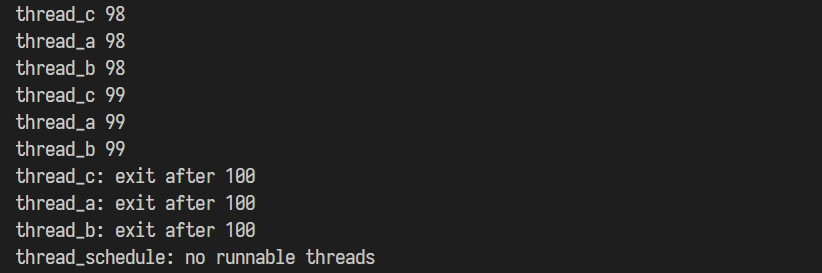
\includegraphics[width=0.8\textwidth]{thread_uthread.jpg}
  \caption{ \lstinline{uthread} 的执行结果}
\end{figure}
说明该用户态线程库的实现是正确的。

\section{线程的使用}

本部分的第二个实验不涉及到 xv6 ,而是在常规的拥有多核的 Linux 机器下进行(需要将我们的虚拟机的 CPU 数量调整为大于 1 的值),使用著名的 \lstinline{pthread} 库来研究多线程中的一些问题。本实验中,我们需要修改 \lstinline{notxv6/ph.c} ,使之在多线程读写一个哈希表的情况下能够产生正确的结果。

首先运行 \lstinline{make ph} 编译 \lstinline{notxv6/ph.c} ,运行 \lstinline{./ph 1} ,可以获得类似下面输出:
\begin{lstlisting}
    100000 puts, 3.991 seconds, 25056 puts/second
    0: 0 keys missing
    100000 gets, 3.981 seconds, 25118 gets/second
\end{lstlisting}

不难发现,写入哈希表的数据被完整地读出,没有遗漏。然后运行 \lstinline{./ph 2} ,则输出如下:
\begin{lstlisting}
    100000 puts, 1.885 seconds, 53044 puts/second
    1: 16579 keys missing
    0: 16579 keys missing
    200000 gets, 4.322 seconds, 46274 gets/second
\end{lstlisting}

在多线程同时读写的情况下,部分数据由于竞争访问,一些数据没有被正确写入到哈希表中,因而我们需要解决这个问题。一个常规的解决方案是给共享数据结构加上锁,获得锁的线程才可以写该数据结构。查阅 \lstinline{man pthreads} 和其它关于 \lstinline{pthread} 的线程加锁的资料后,我们首先定义一个保护哈希表的互斥锁:
\begin{lstlisting}[language=C]
......
    pthread_mutex_t lock;
......
\end{lstlisting}
然后在开始线程前对其进行初始化:
\begin{lstlisting}[language=C]
    pthread_mutex_init(&lock, NULL);
\end{lstlisting}
最后在写入操作哈希表时加上获取锁的操作,并在写入完成后释放锁:
\begin{lstlisting}[language=C]
static 
void put(int key, int value)
{
......
    // the new is new.
    pthread_mutex_lock(&lock);
    insert(key, value, &table[i], table[i]);
    pthread_mutex_unlock(&lock);
......  
}
\end{lstlisting}

此时再使用  \lstinline{make ph} 编译 \lstinline{notxv6/ph.c} ,运行 \lstinline{./ph 2} ,则发现没有读出的数据缺失,如下图所示:
\begin{figure}[H]
  \centering
  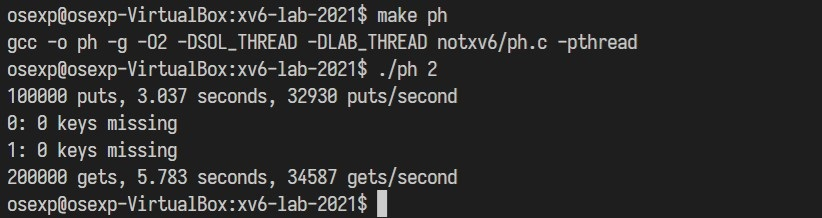
\includegraphics[width=0.8\textwidth]{thread_ph.jpg}
  \caption{ \lstinline{./ph 2} 的执行结果}
\end{figure}

\begin{proposition}[为何读时不加锁] 
    事实上,我们在一些对于数据一致性要求较高的程序(如数据库)中,一个线程在读取数据时,如果不对相应的资源加锁,则可能读到过时或“脏”的数据,这个现象在数据库中被称为“幻读”。数据库根据其需求,设置了各种隔离级别,只有在较高的隔离级别上才会使用加锁或完全串行化操作的方式解决幻读等问题。在上面的 \lstinline{ph} 程序中,由于不涉及到对数据的并发修改或删除,故而在读取时无需加锁。
\end{proposition}

\section{线程屏障}

除了锁以外,线程屏障 \lstinline{barrier} 也是线程进行同步的重要机制。线程屏障 \lstinline{barrier} 可以看成线程的检查点,即某个参与 \lstinline{barrier} 的线程先执行到 \lstinline{barrier()} 语句处时,其需要等待其它尚未到达 \lstinline{barrier()} 处的线程;当所有参与线程屏障的线程都到达 \lstinline{barrier()} 语句处时,所有参与线程屏障的线程都继续运行。

首先运行 \lstinline{make barrier} 编译 \lstinline{notxv6/barrier.c} ,运行 \lstinline{./barrier 2} ,可以获得类似下面输出:
\begin{lstlisting}
    $ make barrier
    $ ./barrier 2
    barrier: notxv6/barrier.c:42: thread: Assertion `i == t' failed.
\end{lstlisting}
说明该 \lstinline{barrier()} 并未正确实现。

根据 xv6 实验手册中的提示,可以使用条件变量来实现 \lstinline{barrier} 机制。首先查看 \lstinline{barrier.c} 中相关的数据结构:
\begin{lstlisting}[language=C]
    struct barrier {
        pthread_mutex_t barrier_mutex;
        pthread_cond_t barrier_cond;
        int nthread;      // Number of threads that have reached this round of the barrier
        int round;     // Barrier round
      } bstate;
\end{lstlisting}

为实现线程屏障,需要维护一个互斥锁、一个条件变量、用以记录到达线程屏障的线程数的整数和记录线程屏障轮数的整数。在初始化用的 \lstinline{barrier_init()} 中,互斥锁、条件变量及 \lstinline{nthread} 被初始化。此后在某个线程到达 \lstinline{barrier()} 时,需要获取互斥锁进而修改 \lstinline{nthread}。当 \lstinline{nthread} 与预定的值相等时,将 \lstinline{nthread} 清零,轮数加一,并唤醒所有等待中的线程。最后不要忘记在 \lstinline{barrier()} 中释放互斥锁。笔者的实现如下所示:
\begin{lstlisting}[language=C]
static void 
barrier()
{
  // YOUR CODE HERE
  pthread_mutex_lock(&bstate.barrier_mutex);
  bstate.nthread ++;
  if (bstate.nthread == nthread)
  {
    bstate.round++;
    bstate.nthread = 0;
    pthread_cond_broadcast(&bstate.barrier_cond);
  } else {
    pthread_cond_wait(&bstate.barrier_cond, &bstate.barrier_mutex);
  }
  pthread_mutex_unlock(&bstate.barrier_mutex);
}
\end{lstlisting}

此时使用 \lstinline{make barrier} 编译 \lstinline{notxv6/barrier.c} ,运行 \lstinline{./barrier 2} ,则通过测试,如下图所示:
\begin{figure}[H]
  \centering
  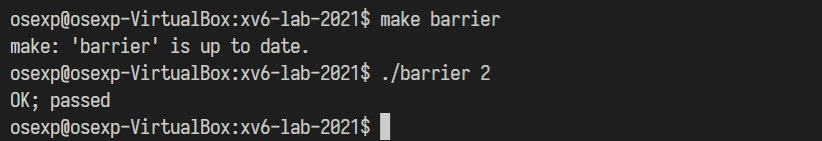
\includegraphics[width=0.8\textwidth]{thread_barrier.jpg}
  \caption{ \lstinline{./barrier 2} 的执行结果}
\end{figure}

\paragraph*{实验结果} 在完成 Lab Multithreading 中的所有实验后,根据 MIT 6.S081 的传统,需要在实验目录下创建一个名为 \lstinline{time.txt} 文本文件,其中只包含一行,为完成该实验的小时数。然后在终端中执行 \lstinline{make grade} ,即可对整个实验进行自动评分,笔者的结果如下:
\begin{figure}[H]
  \centering
  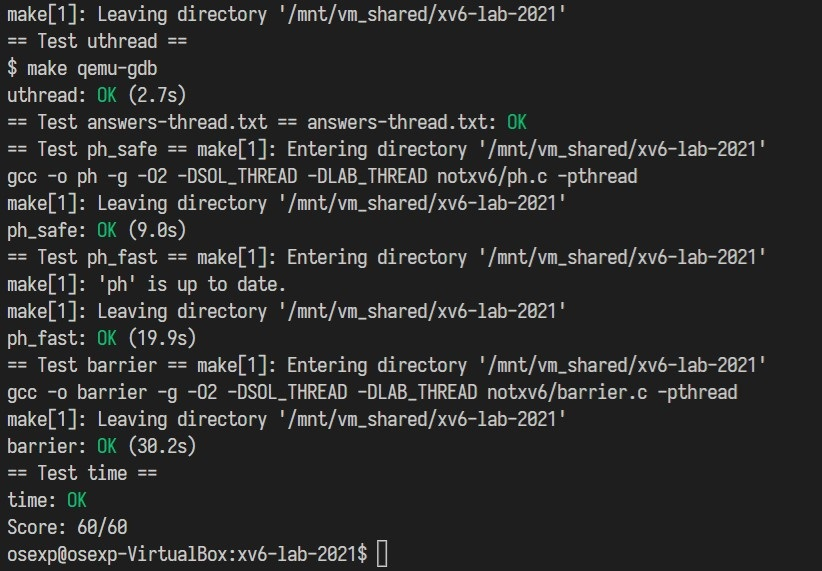
\includegraphics[width=0.8\textwidth]{thread_grade.jpg}
  \caption{ Lab Multithreading 的测评结果}
\end{figure}
可见测试全部通过,得分为满分。

\section{小结:线程、互斥与同步}

Lab Multithreading 中的三个实验并不困难,但是其十分准确地阐释了线程的三个重要概念:上下文切换、互斥与同步。

上下文的切换需要设计存储上下文的数据结构,并在用户态结合 ABI 的规范及使用汇编实现切换程序,从而保存并设置各寄存器(重要的是 ra 和 sp 寄存器)。

由于各线程共享内存空间,在可能发生数据的竞争写入等需要线程互斥的场景,一般使用线程库提供的互斥锁实现线程的互斥。

各线程协作时,可能需要在代码执行到某个位置时使得线程同步,在本部分的实验中,使用条件变量实现的 \lstinline{barrier} 来进行线程同步。

此外,由于线程共享内存空间的特性,线程间通信并不需要特殊的讨论,只需利用内存中共享的数据结构即可完成通信(例如带锁的全局变量等)。

